\scanpage{37}
donne lieu à des applications \uline{étales}
\[ q_n^{-1}(X_i)-q_n^{-1}(X_{i-1})\unsure{\text{---}|\to}X_i-X_{i-1}\qquad(0\leq i\leq n-1) \]

Morphisme d'espaces à $n$-filtrations régulières
\diagram{\begin{tikzcd}[ampersand replacement=\&,row sep=0.1em]f\colon X\arrow[r]\&Y\\[-.4em]\rotatebox{90}{$=$}\&\rotatebox{90}{$=$}\\X_n\&Y_n\\\rotatebox{90}{$\subset$}\&\rotatebox{90}{$\subset$}\\\vdots\&\vdots\end{tikzcd}}
a) $f$ fini
b) $f^{-1}(Y_i)=X_i$ \qquad $(0\leq i\leq n)$
c) $\deleted{\unsure{\forall i|f_i}}.\ X_i-X_{i-1}\unsure{\text{---}|\to}Y_i-Y_{i-1}$ est étale (donc un rev. étale)
% slanted
\margin{\uline{NB} $X_n\mapsto X_i$, $X_n\mapsto\deleted{\unsure{\partial}}\widetilde X_i$, $X_n\mapsto\partial\widetilde X_i$ sont des foncteurs de $\unsure{\mathcal F_n|F_n}$ dans $\mathcal F_i$, $\unsure{\mathcal F_i|\mathcal F_{i-1}}$, \deleted{$\unsure{\mathcal F_i}$} $\mathcal F_{i-1}^{\circ}$ resp. (\unsure{après vérification|vérifiant}). $\partial\widetilde X_i\to X_{i-1}$ \unsure{hom fonctoriel|homéomorphe}\ldots}

Catégorie $\mathcal F_n$ des espaces à $n$-filtrations régulières ss-catégorie pleine \deleted{\unsure{de}} $\mathcal F_n^\circ$ des \deleted{esp} $n$-variétés à $n$-filtr. régulière.

$G_n$ grpe $n$-cartographique (engendré par $\sigma_0\,\sigma_1\ldots\sigma_n$
\[ \begin{aligned}&\text{avec }\sigma_i^2=1\qquad(0\leq i\leq n)\\ &\sigma_i\sigma_j=\sigma_j\sigma_i\quad\text{si }n\geq j\geq i+2,\ i\geq0\\ &\deleted{\unsure{\Longleftrightarrow}}\quad\text{(condition si }n\deleted{\unsure{>}}\geq2) \end{aligned} \]

Par récurrence sur $n$, on va définir des foncteurs
\diagram{\begin{tikzcd}[ampersand replacement=\&]\mathcal F_n^\circ\arrow[r,"E_n^\circ"]\&G_n\text{-ens}\arrow[d,"\text{oubli}"]\&(\uuline{$n\geq1$})\\[-.4em]\rotatebox{90}{$\supset$}\&{}\&{}\\[-.5em]\mathcal F_n\arrow[r,"E_n"]\&G_{n-1}\text{-ens}\&{}\end{tikzcd}}
\diagram{\begin{tikzcd}[ampersand replacement=\&,column sep=small]\widetilde X_1\arrow[d,"{\unsure{p_0|p_1}}"']\&\supset\&\widetilde X_0\arrow[d,"q_0"]=\partial\widetilde X_1\\X_1\&\supset\&X_0\end{tikzcd}}
\textcircled{1} Cas $n=1$ \qquad $\unsure{E_n^\circ|E_n}(X_1)=\pi_0(\underbrace{\widetilde X_1^{\mathrm{or}}}_{\substack{\text{rev. orienté}\\\text{de }\widetilde X_1}})={}$ ens des arcs de $X_1$ $=\partial\widetilde X_1$
\deleted{= \unsure{ensemble, couples} $(\unsure{a_0,a_1}),\ldots$} \deleted{$\sigma_0$ = changement d'orientation} \deleted{\illegible{1}} \deleted{$\unsure{\sigma_1(x)}$}
\deleted{$a_0\in\partial\widetilde X_1,\ a_1\in\pi_0(\widetilde X_1),\ a_0\in a_1$}
\figure{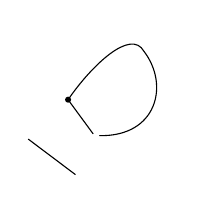
\begin{tikzpicture}[scale=.55]\fill (0,0) circle(.07);\draw (0,0).. controls (.55,.8) and (1.45,1.65) .. (1.75,1.12).. controls (2.35,.34) and (2.05,-.86) ..(.72,-.83);\draw (.58,-.79)--(0,0);\draw (-.92,-.91)--(.17,-1.73);\end{tikzpicture}}
\deleted{$\sigma_0={}$ chg$^{t}$ d'orientation} \deleted{échangeant les p$^{\rm ts}$ des fibres de} \deleted{\unsure{la projection} $\unsure{\sigma_1(a_0,a_1)=(a'_0,a_1)}$} \deleted{$a'_0\ne a_0$}
\deleted{$F_n^\circ(X_1)=\partial\widetilde X_1\to\pi_0(\partial\widetilde X_1)$} \deleted{$\sigma_1(a_0)\unsure{=}(a'_0\unsure{,a'_1})$ avec $q_0(a_0)=q_0(a'_0)$ $a'_0\ne a_0$} \deleted{$q_0(a_0)=q_0(a'_0)$} \deleted{échange les p$^{\rm ts}$ des fibres de $\partial\widetilde X_1\to X_0$}
% archive sheet number: 36
